% CS F407 Artificial Intelligence: final project report template.
% Limit: 2 pages, including everything except references.
% Do not change the font size, margins or spacing.
\documentclass[11pt,a4paper,twocolumn]{article}

\usepackage[margin=2cm,columnsep=0.8cm]{geometry}
\usepackage[T1]{fontenc}
\usepackage{lmodern}
\usepackage{microtype}
\usepackage{amsmath,amssymb}
\usepackage{graphicx}
\usepackage{booktabs}
\usepackage{tabularx}
\usepackage{enumitem}
\usepackage{titlesec}
\usepackage[hidelinks]{hyperref}

\titleformat{\section}{\normalsize\bfseries}{\thesection}{0.6em}{}
\titlespacing*{\section}{0pt}{1.2ex plus 0.3ex}{0.6ex}
\setlist{nosep,leftmargin=*}
\setlength{\parskip}{0.3ex}

\newcommand{\coursename}{CS F407 Artificial Intelligence, AY 2026--27 Semester I}
\newcommand{\teamno}{Made by Claude}
\newcommand{\githuburl}{https://github.com/green-turtle18/dna-lang}

\begin{document}

\twocolumn[{%
\begin{center}
  {\large\bfseries Can AI Read the Language of DNA? Separating Disease Genes from Non-Disease Genes Using Only Their Coding Sequence}\\[1ex]
  \teamno\\
  Dev Raman Taneja (2023A7PS0336G), Leora Modi (2023B4AD0866G),\\ Nidhi Deepak Mekaraj (2024A7PS0014G), Pranay Pankaj Ghumatkar (2024A3PS0328G)\\[0.5ex]
  {\small \coursename, BITS Pilani, K.K. Birla Goa Campus}\\[1.5ex]
  \begin{minipage}{0.85\textwidth}
    \small
    \centerline{\bfseries Abstract}\vspace{0.5ex}
    We treat DNA as a text written in a four-letter alphabet and ask whether
    language-processing methods can tell human disease genes from genes with no
    known disease link. We built a curated dataset of 15,665 human protein-coding
    sequences (4,483 disease, 11,182 non-disease) and compared k-mer bag-of-words,
    TF-IDF, word2vec and a small pretrained transformer, with logistic regression,
    random forests and neural networks. Disease genes are longer, so length alone
    scores ROC-AUC 0.62. On a test split where length and GC content are matched,
    the length control falls to chance (0.48) while sequence models reach 0.60, and
    0.56 after removing all base-composition information. The models read real
    structure: word2vec recovers the genetic code from context alone. Finally, we
    checked 36 testable explanations generated by three AI chatbots against the
    data; broad explanations held up, and specific, confident ones often failed.
  \end{minipage}
\end{center}
\vspace{1.5ex}
}]

\section{Introduction}
A gene's coding sequence is a string over $\{A,C,G,T\}$. If we treat it as text,
can methods from natural language processing learn its vocabulary, grammar and
context well enough to recognise genes associated with human disease?
The \emph{input} to our system is the coding sequence of one human gene; the
\emph{output} is the probability that the gene is a Mendelian disease gene.

The difficulty is knowing what a classifier has learned: disease genes differ
from other genes in simple ways, such as length, that a model can exploit without
reading any ``language''. Our contributions are:
(i) a curated, documented disease vs non-disease gene dataset with
homology-aware and length/GC-matched splits;
(ii) a systematic comparison of text representations and models from
bag-of-words to a pretrained transformer;
(iii) control experiments that separate genuine sequence signal from
length and composition artefacts; and
(iv) a protocol that turns AI-generated explanations into statistical tests.

\section{Background and related work}
\textbf{Sequence as text.} Splitting a sequence into overlapping $k$-mers turns
it into a document of ``words'', which supports bag-of-words and TF-IDF
features~\cite{russell2021aima}. word2vec~\cite{mikolov2013} learns word vectors
from co-occurrence in a context window; dna2vec~\cite{ng2017dna2vec} applies it to
$k$-mers. DNABERT~\cite{ji2021dnabert} pretrains a BERT-style
transformer~\cite{devlin2019bert} on the human genome with a masked-token
objective and fine-tunes it for downstream tasks.

\textbf{Disease genes.} Disease genes differ from other genes in length,
conservation and paralogy~\cite{lopezbigas2004}. CpG sites mutate about ten
times faster than other sites~\cite{hodgkinson2011}, which affects which genes
acquire pathogenic variants. Gene--disease links come from OMIM via the Human
Phenotype Ontology (HPO)~\cite{gargano2024hpo}.

\section{Method}
\textbf{Dataset.} Sequences are full-length human open reading frames (ORFs) from the
ORFeome~9.1 collection~\cite{orfeome2016}, one per gene. We kept ORFs that are
ACGT-only, start with ATG, have a length divisible by three, are at least 150\,nt
and have no internal stop codon; exact duplicates and non-protein-coding entries
were removed, and the terminal stop codon was stripped so that its presence
could not act as a cloning artefact. A gene is labelled \emph{disease} (1) if HPO
(release 2026-09-01) lists at least one OMIM Mendelian gene--phenotype link, and
\emph{non-disease} (0) if it appears in no source at all: HPO (OMIM or Orphanet,
any association type), ClinVar pathogenic genes, curated OMIM, ClinGen and
haploinsufficiency lists, and clinical panels. The 782 genes with only weak
evidence were set aside rather than labelled.

\textbf{Splits.} \emph{random}: stratified 80/20. \emph{family}: 80/20 with
paralogs kept on one side; proteins sharing $\ge$10 amino-acid 5-mers covering
$\ge$20\% of the shorter protein are linked, and connected components form
families. \emph{lenmatch}: the family split restricted to a balanced subset of
8,902 genes in which both classes have the same joint length\,$\times$\,GC
histogram. \emph{lenmatch} is our headline split, because there length and
GC cannot explain any result.

\textbf{Representations.}
(1) Overlapping $k$-mers ($k{=}3,4,6$ and $3$--$6$) and non-overlapping in-frame
codons, as raw counts or TF-IDF, with the vocabulary fitted on training genes only.
(2) word2vec skip-gram~\cite{mikolov2013} on codons (32-d) and 6-mers (64-d),
trained on training genes only; a gene vector is the mean of its word vectors.
(3) A 2-layer transformer (64-d, 4 heads, 92k parameters) over codon tokens,
pretrained with BERT-style masked-codon prediction (15\% of codons hidden) on
training genes and then fine-tuned with a classification head; genes are read
in 256-codon windows whose predictions are averaged. We also trained it without
pretraining.

\textbf{Models.} Logistic regression, random forest (200 trees) and an MLP
(one hidden layer of 128 units, early stopping). Only 29\% of genes are disease
genes, so unweighted models predicted ``non-disease'' for everything; we use
balanced class weights (LR, RF), oversampling of the training set (MLP) and a
weighted loss (transformer).

\textbf{Controls and interpretation.} (a) Length and GC-only models.
(b) Bases shuffled within each gene. (c) Models restricted to one kind of
information: CpG observed/expected, dinucleotides, amino-acid composition, or
relative synonymous codon usage (RSCU, which removes the protein). (d) Synonymous
shuffling: each codon is replaced by a random synonym, keeping the protein.
(e) Composition regression: codon frequencies minus a linear prediction from GC at
each codon position, CpG and all 16 dinucleotides, fitted on training genes.

\textbf{LLM explanations.} We gave Claude (Opus 5.5), ChatGPT and Gemini
(web versions, November 2026) the same fixed prompt summarising our patterns
and asked for biological explanations, testable predictions and likely artefacts.
Each specific claim was converted into a per-gene statistic and tested on the
lenmatch subset with a Mann--Whitney $U$ test and Benjamini--Hochberg false
discovery rate; claims needing data we do not have (expression, methylation,
publication counts) were recorded as untestable.

\section{Experimental setup}
The data are 15,665 genes: 4,483 disease, 11,182 non-disease (median length 1,425
vs 1,074\,nt; mean GC 0.529 vs 0.527). Test sets have 3,134 genes (random,
family) and 1,797 (lenmatch). The main metric is ROC-AUC (higher is better; 0.5
is chance), with macro-F1 as a secondary metric. 95\% confidence intervals come
from 1,000 bootstrap resamples of the test set; on lenmatch the interval is about
$\pm$0.026. All runs use seed 0. Software: Python with scikit-learn, SciPy,
gensim (word2vec) and PyTorch (transformer); everything ran on a 2-core CPU.

\section{Results}
\begin{table*}[t]
\centering
\small
\begin{tabular}{lcccccc}
\toprule
 & \multicolumn{3}{c}{family split (paralogs apart)} & \multicolumn{3}{c}{lenmatch split (length \& GC matched)} \\
\cmidrule(lr){2-4}\cmidrule(lr){5-7}
Representation & LR & RF & MLP & LR & RF & MLP \\
\midrule
Control: length + GC & 0.615 & 0.569 & -- & 0.488 & 0.478 & -- \\
TF-IDF, $k=3$ & 0.623 & 0.652 & 0.632 & 0.578 & 0.584 & 0.580 \\
TF-IDF, $k=4$ & 0.643 & \textbf{0.661} & 0.610 & 0.585 & 0.597 & 0.582 \\
TF-IDF, $k=6$ & 0.635 & 0.642 & 0.574 & 0.569 & 0.567 & 0.577 \\
TF-IDF, $k=3$--$6$ & 0.651 & 0.655 & 0.570 & 0.584 & 0.580 & 0.577 \\
TF-IDF, codons & 0.635 & \textbf{0.661} & 0.638 & \textbf{0.599} & 0.592 & 0.570 \\
word2vec mean, codons & 0.588 & 0.638 & 0.646 & 0.584 & \textbf{0.600} & 0.576 \\
word2vec mean, 6-mers & 0.598 & 0.655 & 0.601 & 0.573 & 0.592 & 0.587 \\
\midrule
Transformer, pretrained & \multicolumn{3}{c}{0.630} & \multicolumn{3}{c}{0.587} \\
Transformer, no pretraining & \multicolumn{3}{c}{--} & \multicolumn{3}{c}{0.579} \\
\bottomrule
\end{tabular}
\caption{Test ROC-AUC (higher is better; 0.5 is chance) for every representation
and model on the two honest splits. Differences below about 0.03 are within the
95\% confidence interval. On the random split the best AUC is 0.666, almost the
same as on the family split, so paralog leakage does not inflate the results.}
\label{tab:results}
\end{table*}

\textbf{Length explains the easy wins.} With length and GC alone, logistic
regression reaches 0.615 on the family split (Fig.~\ref{fig:honest}). Once length
and GC are matched (lenmatch), this control falls to chance (0.478--0.488), while
sequence models keep an AUC of 0.57--0.60 (Table~\ref{tab:results}). Shuffling
bases within each gene drops $k{=}6$ models to chance (0.49--0.51), so the order
of bases, not only their counts, carries the signal.

\begin{figure}[t]
\centering
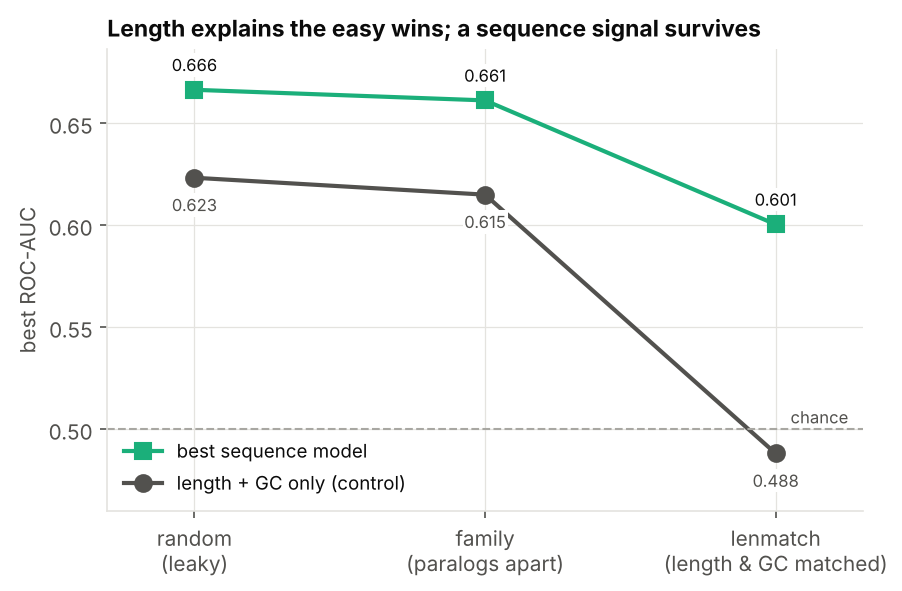
\includegraphics[width=0.82\linewidth]{figures/summary_leaky_to_honest.png}
\caption{Best sequence model vs the length+GC control as the split gets harder.}
\label{fig:honest}
\end{figure}

\textbf{Representations and models.} Larger $k$ does not help: $k{=}6$ (4,096
features) is no better than $k{=}4$ (256), and the MLP overfits large
vocabularies. In-frame codons are at or near the top with only 61 features. The
top five lenmatch models lie within 0.01 of each other; we select TF-IDF codons
with logistic regression (AUC 0.599, macro-F1 0.562), the simplest and most
interpretable. Neither the MLP nor the transformer beats the linear models, and
masked-codon pretraining did not measurably help (0.587 vs 0.579).

\textbf{What the models learned.} Both the protein and its codon ``spelling''
carry signal (Fig.~\ref{fig:features}): amino-acid composition alone gives 0.578,
synonymous codon choice alone (protein removed) 0.573, and full codon usage 0.598.
Removing all composition information (GC at each codon position, CpG,
dinucleotides) lowers codon usage from 0.598 to 0.558 [0.529, 0.587]. About 40\%
of the signal above chance is therefore compositional, and the rest survives.
Disease genes are less CpG-depleted than non-disease genes (CpG
observed/expected 0.467 vs 0.438, $p<10^{-6}$), prefer CG-containing arginine
codons (CGT, CGC over AGA, AGG) and contain fewer cysteines, a residue that is
common in the large zinc-finger gene family, which is mostly non-disease.
Removing the zinc-finger, olfactory-receptor and keratin-associated families
shrinks the cysteine effect from $-0.18$ to $-0.07$ (log$_2$ ratio) but leaves
the AUC almost unchanged (0.598 to 0.586).

\begin{figure}[t]
\centering
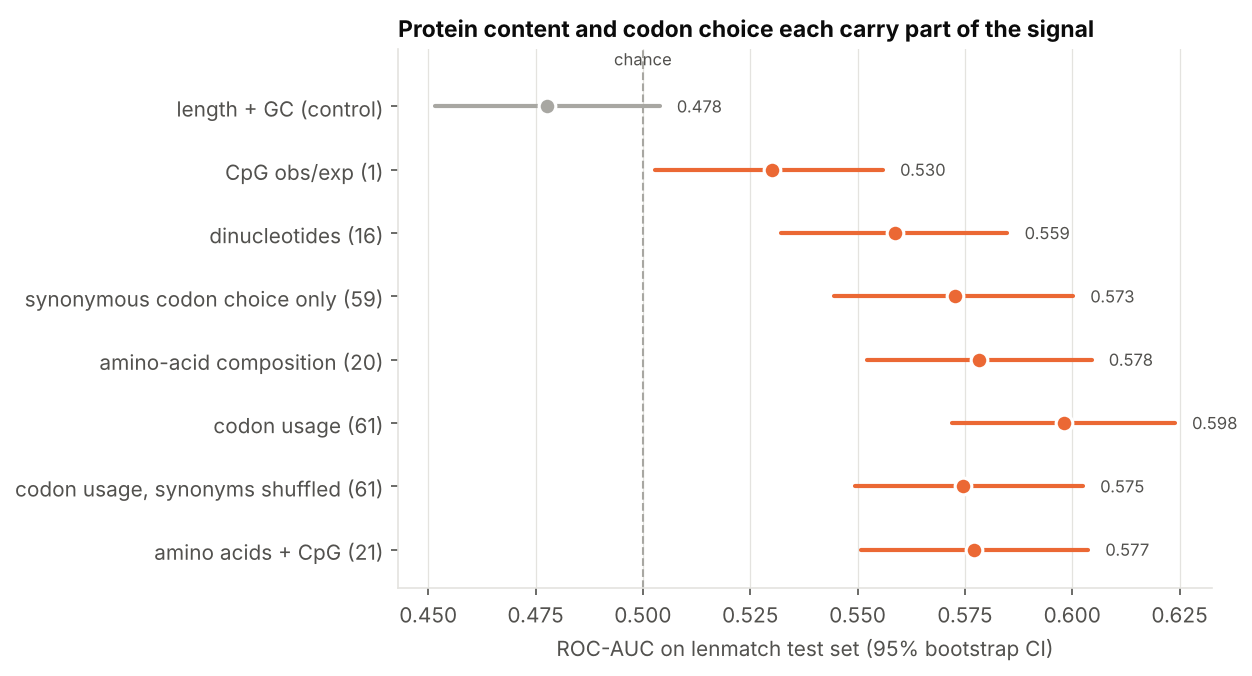
\includegraphics[width=0.9\linewidth]{figures/interpret_feature_sets.png}
\caption{Lenmatch AUC (95\% CI) for models restricted to one kind of information.}
\label{fig:features}
\end{figure}

\textbf{Vocabulary and context.} Both classes share almost the same vocabulary
(Spearman $\rho=0.995$ for 6-mer frequencies). The rarest 6-mers expose two
``grammar rules'': 92\% contain CG (CpG avoidance) and many contain stop codons,
which cannot occur in frame. word2vec, never told the genetic code,
places synonymous codons closer together than non-synonymous pairs (mean cosine
0.85 vs 0.71, permutation $p=0.0005$). Synonyms stay closer even when their third
bases differ (0.83 vs 0.75 for non-synonyms sharing a third base), and 57\% of codons have a synonym as their
nearest neighbour, against 5\% by chance. Shuffling codon order within genes
halves this effect, so about half comes from local context, which bag-of-words
cannot capture. The transformer's codon embeddings mostly encoded third-base GC.

\textbf{LLM explanations.} Of 36 testable claims, 8 of 13 held for
Claude (which also helped build the analysis, so its score is not blind), 5 of 11
plus one partly for ChatGPT, and 3 of 12 for Gemini, with 2 of Gemini's in the
\emph{opposite} direction (FDR 5\%). All three systems named the same core mechanisms (CpG mutability and
ascertainment, gene families, protein class), and each also proposed specific
mechanisms that the data rejected. Gemini, the most specific and confident,
predicted that the CpG excess would sit at protein-changing positions near the
5$'$ end; it is strongest at sites that include the synonymous third position and
persists along the whole gene. ChatGPT's main alternative explanation (GC-biased
gene conversion raising GC3) was not supported, but its suggested control
(composition regression) was the most useful contribution of any system.

\section{Discussion and limitations}
A text model can detect a weak but genuine disease-associated signal in coding
DNA. The signal is not an artefact of length, GC content or paralog leakage, and
it is interpretable: CpG content, codon choice and protein composition. It is
weak because most of what makes a gene cause disease (its function, dosage
sensitivity and tissue of expression) is not written in its coding sequence.

\emph{Limitations.} ``Non-disease'' means ``no disease link known yet'', so some
negatives are undiscovered disease genes. Part of the signal may reflect
ascertainment: well-studied and CpG-rich (more mutable) genes are found sooner.
The ORFeome lacks very long genes (e.g.\ TTN), and we used one seed per split.
Our transformer is small and CPU-trained, not the pretrained
DNABERT~\cite{ji2021dnabert}. Next steps: fine-tune DNABERT on a GPU, and match
genes on expression and publication counts to measure ascertainment bias.

\section{Conclusion}
DNA does behave like a language that models can learn from. word2vec rediscovers
the genetic code from context, and rare words reveal grammar rules. With that
language, models separate disease genes from non-disease genes better than
chance (AUC 0.60 with length and GC matched), but only modestly. AI-generated
explanations are best treated as hypotheses: between a quarter and about 60\% of
each system's specific claims survived testing.

\section*{Individual member contributions}
{\small
\begin{tabularx}{\linewidth}{@{}>{\raggedright}p{2.1cm} >{\raggedright\arraybackslash}X@{}}
\toprule
Name & Contribution \\
\midrule
Dev Raman Taneja & Representations: $k$-mer, codon and TF-IDF features,
vocabulary analysis and word2vec embeddings; collected the ChatGPT and Gemini
explanations. \\
Leora Modi & Data: disease dataset curation, labels and the three splits;
gene-family data loading; the codon transformer; repository maintenance. \\
Nidhi Deepak Mekaraj & Controls and interpretation: length, GC and shuffle
controls, composition analyses, and verification of the LLM explanations. \\
Pranay Pankaj Ghumatkar & Models and evaluation: logistic regression, random
forest and MLP experiments, class-imbalance handling, the combined comparison
and final model selection. \\
\bottomrule
\end{tabularx}}

\smallskip
\noindent Every member ran the full pipeline end to end and verified the
reported results. All members have read this report and agree with the
statement above.

\section*{Generative AI disclosure}
All code in this project, both before and after the midsem, was written by
generative AI: Claude (Anthropic), using Claude Opus 5.5 for the second half.
This covers the dataset pipeline, representations, models, controls,
analysis modules and figures. Claude also drafted the documentation and this
report. Every team member ran the code, checked that it reproduces the
reported numbers, and reviewed the text; we take responsibility for all of
it. ChatGPT and Gemini were used only as subjects of the LLM-explanation
experiment (Section~3).

\section*{Code availability}
\noindent Code and data:\\
\url{\githuburl}\\
The README gives the commands to reproduce every result; \texttt{docs/findings.md}
maps each result to its source file.

\begin{thebibliography}{9}
\small
\bibitem{russell2021aima}
S.~Russell and P.~Norvig.
\newblock \emph{Artificial Intelligence: A Modern Approach}, 4th edition.
\newblock Pearson, 2021.

\bibitem{mikolov2013}
T.~Mikolov, K.~Chen, G.~Corrado and J.~Dean.
\newblock Efficient estimation of word representations in vector space.
\newblock \emph{arXiv:1301.3781}, 2013.

\bibitem{ng2017dna2vec}
P.~Ng.
\newblock dna2vec: Consistent vector representations of variable-length
  $k$-mers.
\newblock \emph{arXiv:1701.06279}, 2017.

\bibitem{devlin2019bert}
J.~Devlin, M.-W.~Chang, K.~Lee and K.~Toutanova.
\newblock BERT: Pre-training of deep bidirectional transformers for language
  understanding.
\newblock In \emph{Proc.\ NAACL-HLT}, 2019.

\bibitem{ji2021dnabert}
Y.~Ji, Z.~Zhou, H.~Liu and R.~V.~Davuluri.
\newblock DNABERT: pre-trained bidirectional encoder representations from
  transformers model for DNA-language in genome.
\newblock \emph{Bioinformatics}, 37(15):2112--2120, 2021.

\bibitem{lopezbigas2004}
N.~L\'opez-Bigas and C.~A.~Ouzounis.
\newblock Genome-wide identification of genes likely to be involved in human
  genetic disease.
\newblock \emph{Nucleic Acids Research}, 32(10):3108--3114, 2004.

\bibitem{hodgkinson2011}
A.~Hodgkinson and A.~Eyre-Walker.
\newblock Variation in the mutation rate across mammalian genomes.
\newblock \emph{Nature Reviews Genetics}, 12:756--766, 2011.

\bibitem{gargano2024hpo}
M.~A.~Gargano et al.
\newblock The Human Phenotype Ontology in 2024: phenotypes around the world.
\newblock \emph{Nucleic Acids Research}, 52(D1):D1333--D1346, 2024.

\bibitem{orfeome2016}
The ORFeome Collaboration.
\newblock The ORFeome Collaboration: a genome-scale human ORF-clone resource.
\newblock \emph{Nature Methods}, 13:191--192, 2016.
\end{thebibliography}

\end{document}
